\documentclass[border=3pt]{standalone}
% Preâmbulo compartilhado pelos diagramas TikZ da aula 4 de Navegação (Representação de Mapas)
\usepackage[T1]{fontenc}
\usepackage[utf8]{inputenc}
\usepackage{lmodern}
\usepackage{amsmath}
\usepackage{xcolor}
\usepackage{tikz}
\usetikzlibrary{arrows.meta,angles,quotes,decorations.pathmorphing,decorations.pathreplacing,calc,
                positioning,shapes.geometric,shapes.misc,backgrounds,fit,
                math}

% Paleta (mesma dos SVGs originais)
\definecolor{dblue}{HTML}{2A5B8C}
\definecolor{dorange}{HTML}{B3541E}
\definecolor{dgreen}{HTML}{4A7C59}
\definecolor{dred}{HTML}{9C4B4B}
\definecolor{dcream}{HTML}{F4F1EA}
\definecolor{dshade}{HTML}{DDD7C9}

% Função gaussiana (não normalizada por padrão de escala visual)
\pgfmathdeclarefunction{gauss}{3}{%
  \pgfmathparse{1/(#3*sqrt(2*pi))*exp(-((#1-#2)^2)/(2*#3^2))}%
}

% Estilos comuns (prefixo d... para não colidir com chaves internas do pgf)
\tikzset{
  >={Stealth[length=2mm]},
  dguide/.style={gray!55, dashed, line width=0.4pt},
  daxis/.style={gray!60, line width=0.7pt, ->},
  dbody/.style={fill=black!3, draw=black!80, line width=1pt},
  dacc/.style={draw=dblue, line width=1pt},
  dlbl/.style={black!55, font=\small},
  dsub/.style={black!45, font=\footnotesize},
  dstate/.style={circle, draw=black!80, fill=dcream, line width=1pt,
                 minimum size=17mm, font=\large, inner sep=1pt},
  dobs/.style={circle, draw=black!80, fill=dshade, line width=1pt,
               minimum size=14mm, font=\large, inner sep=1pt},
  dbox/.style={rounded corners=2pt, draw=black!80, fill=dcream, line width=1pt,
               align=center, inner sep=6pt},
  dop/.style={circle, draw=black!80, fill=white, line width=1pt,
              minimum size=6mm, inner sep=0pt, font=\small},
  dtrans/.style={->, dblue, line width=1pt},
  dmeas/.style={->, dorange, line width=1pt},
  dcurve/.style={line width=1pt, dblue},
  dcurveb/.style={line width=1.4pt, dorange},
}

\begin{document}
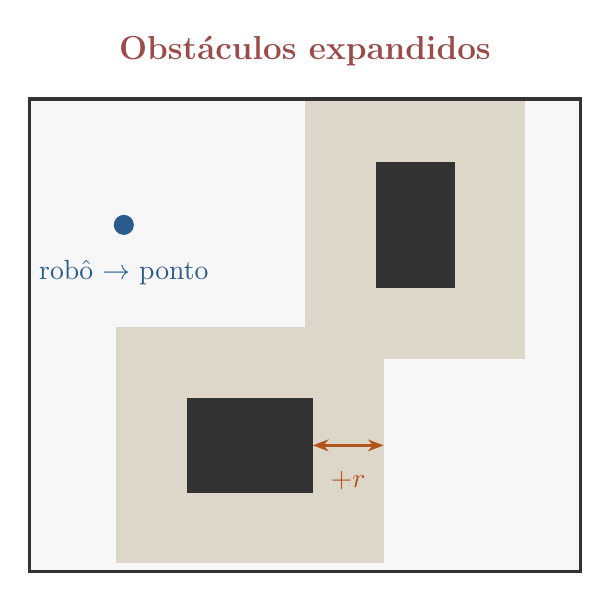
\begin{tikzpicture}[x=1cm,y=1cm]
  \draw[dbody, line width=1.2pt] (0,0) rectangle (7,6);
  \node[font=\bfseries\large, dred] at (3.5,6.6) {Obstáculos expandidos};
  \begin{scope}
    \clip (0,0) rectangle (7,6);
    \fill[dshade] (2.0-0.9,1.0-0.9) rectangle (3.6+0.9,2.2+0.9);
    \fill[dshade] (4.4-0.9,3.6-0.9) rectangle (5.4+0.9,5.2+0.9);
  \end{scope}
  \fill[black!80] (2.0,1.0) rectangle (3.6,2.2);
  \fill[black!80] (4.4,3.6) rectangle (5.4,5.2);
  \draw[black!80, fill=none, line width=1.2pt] (0,0) rectangle (7,6);
  \node[draw=dblue, fill=dblue, circle, minimum size=2.4mm, inner sep=0pt] at (1.2,4.4) {};
  \node[dblue, font=\normalsize] at (1.2,3.8) {robô $\to$ ponto};
  \draw[dorange, line width=1pt, <->] (3.6,1.6) -- (3.6+0.9,1.6);
  \node[dorange, font=\normalsize] at (4.05,1.15) {$+r$};
\end{tikzpicture}
\end{document}
